\documentclass[1p]{elsarticle_modified}
%\bibliographystyle{elsarticle-num}

%\usepackage[colorlinks]{hyperref}
%\usepackage{abbrmath_seonhwa} %\Abb, \Ascr, \Acal ,\Abf, \Afrak
\usepackage{amsfonts}
\usepackage{amssymb}
\usepackage{amsmath}
\usepackage{amsthm}
\usepackage{scalefnt}
\usepackage{amsbsy}
\usepackage{kotex}
\usepackage{caption}
\usepackage{subfig}
\usepackage{color}
\usepackage{graphicx}
\usepackage{xcolor} %% white, black, red, green, blue, cyan, magenta, yellow
\usepackage{float}
\usepackage{setspace}
\usepackage{hyperref}

\usepackage{tikz}
\usetikzlibrary{arrows}

\usepackage{multirow}
\usepackage{array} % fixed length table
\usepackage{hhline}

%%%%%%%%%%%%%%%%%%%%%
\makeatletter
\renewcommand*\env@matrix[1][\arraystretch]{%
	\edef\arraystretch{#1}%
	\hskip -\arraycolsep
	\let\@ifnextchar\new@ifnextchar
	\array{*\c@MaxMatrixCols c}}
\makeatother %https://tex.stackexchange.com/questions/14071/how-can-i-increase-the-line-spacing-in-a-matrix
%%%%%%%%%%%%%%%

\usepackage[normalem]{ulem}

\newcommand{\msout}[1]{\ifmmode\text{\sout{\ensuremath{#1}}}\else\sout{#1}\fi}
%SOURCE: \msout is \stkout macro in https://tex.stackexchange.com/questions/20609/strikeout-in-math-mode

\newcommand{\cancel}[1]{
	\ifmmode
	{\color{red}\msout{#1}}
	\else
	{\color{red}\sout{#1}}
	\fi
}

\newcommand{\add}[1]{
	{\color{blue}\uwave{#1}}
}

\newcommand{\replace}[2]{
	\ifmmode
	{\color{red}\msout{#1}}{\color{blue}\uwave{#2}}
	\else
	{\color{red}\sout{#1}}{\color{blue}\uwave{#2}}
	\fi
}

\newcommand{\Sol}{\mathcal{S}} %segment
\newcommand{\D}{D} %diagram
\newcommand{\A}{\mathcal{A}} %arc


%%%%%%%%%%%%%%%%%%%%%%%%%%%%%5 test

\def\sl{\operatorname{\textup{SL}}(2,\Cbb)}
\def\psl{\operatorname{\textup{PSL}}(2,\Cbb)}
\def\quan{\mkern 1mu \triangleright \mkern 1mu}

\theoremstyle{definition}
\newtheorem{thm}{Theorem}[section]
\newtheorem{prop}[thm]{Proposition}
\newtheorem{lem}[thm]{Lemma}
\newtheorem{ques}[thm]{Question}
\newtheorem{cor}[thm]{Corollary}
\newtheorem{defn}[thm]{Definition}
\newtheorem{exam}[thm]{Example}
\newtheorem{rmk}[thm]{Remark}
\newtheorem{alg}[thm]{Algorithm}

\newcommand{\I}{\sqrt{-1}}
\begin{document}

%\begin{frontmatter}
%
%\title{Boundary parabolic representations of knots up to 8 crossings}
%
%%% Group authors per affiliation:
%\author{Yunhi Cho} 
%\address{Department of Mathematics, University of Seoul, Seoul, Korea}
%\ead{yhcho@uos.ac.kr}
%
%
%\author{Seonhwa Kim} %\fnref{s_kim}}
%\address{Center for Geometry and Physics, Institute for Basic Science, Pohang, 37673, Korea}
%\ead{ryeona17@ibs.re.kr}
%
%\author{Hyuk Kim}
%\address{Department of Mathematical Sciences, Seoul National University, Seoul 08826, Korea}
%\ead{hyukkim@snu.ac.kr}
%
%\author{Seokbeom Yoon}
%\address{Department of Mathematical Sciences, Seoul National University, Seoul, 08826,  Korea}
%\ead{sbyoon15@snu.ac.kr}
%
%\begin{abstract}
%We find all boundary parabolic representation of knots up to 8 crossings.
%
%\end{abstract}
%\begin{keyword}
%    \MSC[2010] 57M25 
%\end{keyword}
%
%\end{frontmatter}

%\linenumbers
%\tableofcontents
%
\newcommand\colored[1]{\textcolor{white}{\rule[-0.35ex]{0.8em}{1.4ex}}\kern-0.8em\color{red} #1}%
%\newcommand\colored[1]{\textcolor{white}{ #1}\kern-2.17ex	\textcolor{white}{ #1}\kern-1.81ex	\textcolor{white}{ #1}\kern-2.15ex\color{red}#1	}

{\Large $\underline{12a_{0758}~(K12a_{0758})}$}

\setlength{\tabcolsep}{10pt}
\renewcommand{\arraystretch}{1.6}
\vspace{1cm}\begin{tabular}{m{100pt}>{\centering\arraybackslash}m{274pt}}
\multirow{5}{120pt}{
	\centering
	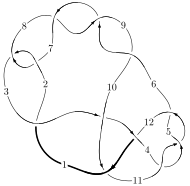
\includegraphics[width=112pt]{../../../GIT/diagram.site/Diagrams/png/1559_12a_0758.png}\\
\ \ \ A knot diagram\footnotemark}&
\allowdisplaybreaks
\textbf{Linearized knot diagam} \\
\cline{2-2}
 &
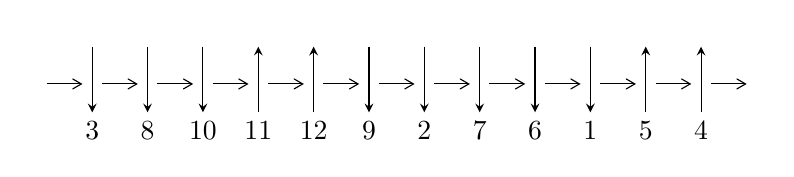
\begin{tikzpicture}[x=20pt, y=17pt]
	% nodes
	\node (C0) at (0, 0) {};
	\node (C1) at (1, 0) {};
	\node (C1U) at (1, +1) {};
	\node (C1D) at (1, -1) {3};

	\node (C2) at (2, 0) {};
	\node (C2U) at (2, +1) {};
	\node (C2D) at (2, -1) {8};

	\node (C3) at (3, 0) {};
	\node (C3U) at (3, +1) {};
	\node (C3D) at (3, -1) {10};

	\node (C4) at (4, 0) {};
	\node (C4U) at (4, +1) {};
	\node (C4D) at (4, -1) {11};

	\node (C5) at (5, 0) {};
	\node (C5U) at (5, +1) {};
	\node (C5D) at (5, -1) {12};

	\node (C6) at (6, 0) {};
	\node (C6U) at (6, +1) {};
	\node (C6D) at (6, -1) {9};

	\node (C7) at (7, 0) {};
	\node (C7U) at (7, +1) {};
	\node (C7D) at (7, -1) {2};

	\node (C8) at (8, 0) {};
	\node (C8U) at (8, +1) {};
	\node (C8D) at (8, -1) {7};

	\node (C9) at (9, 0) {};
	\node (C9U) at (9, +1) {};
	\node (C9D) at (9, -1) {6};

	\node (C10) at (10, 0) {};
	\node (C10U) at (10, +1) {};
	\node (C10D) at (10, -1) {1};

	\node (C11) at (11, 0) {};
	\node (C11U) at (11, +1) {};
	\node (C11D) at (11, -1) {5};

	\node (C12) at (12, 0) {};
	\node (C12U) at (12, +1) {};
	\node (C12D) at (12, -1) {4};
	\node (C13) at (13, 0) {};

	% arrows
	\draw[->,>={angle 60}]
	(C0) edge (C1) (C1) edge (C2) (C2) edge (C3) (C3) edge (C4) (C4) edge (C5) (C5) edge (C6) (C6) edge (C7) (C7) edge (C8) (C8) edge (C9) (C9) edge (C10) (C10) edge (C11) (C11) edge (C12) (C12) edge (C13) ;	\draw[->,>=stealth]
	(C1U) edge (C1D) (C2U) edge (C2D) (C3U) edge (C3D) (C4D) edge (C4U) (C5D) edge (C5U) (C6U) edge (C6D) (C7U) edge (C7D) (C8U) edge (C8D) (C9U) edge (C9D) (C10U) edge (C10D) (C11D) edge (C11U) (C12D) edge (C12U) ;
	\end{tikzpicture} \\
\hhline{~~} \\& 
\textbf{Solving Sequence} \\ \cline{2-2} 
 &
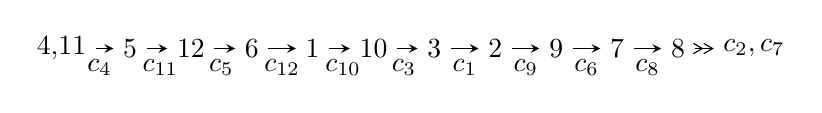
\begin{tikzpicture}[x=22pt, y=7pt]
	% node
	\node (A0) at (-1/8, 0) {4,11};
	\node (A1) at (1, 0) {5};
	\node (A2) at (2, 0) {12};
	\node (A3) at (3, 0) {6};
	\node (A4) at (4, 0) {1};
	\node (A5) at (5, 0) {10};
	\node (A6) at (6, 0) {3};
	\node (A7) at (7, 0) {2};
	\node (A8) at (8, 0) {9};
	\node (A9) at (9, 0) {7};
	\node (A10) at (10, 0) {8};
	\node (C1) at (1/2, -1) {$c_{4}$};
	\node (C2) at (3/2, -1) {$c_{11}$};
	\node (C3) at (5/2, -1) {$c_{5}$};
	\node (C4) at (7/2, -1) {$c_{12}$};
	\node (C5) at (9/2, -1) {$c_{10}$};
	\node (C6) at (11/2, -1) {$c_{3}$};
	\node (C7) at (13/2, -1) {$c_{1}$};
	\node (C8) at (15/2, -1) {$c_{9}$};
	\node (C9) at (17/2, -1) {$c_{6}$};
	\node (C10) at (19/2, -1) {$c_{8}$};
	\node (A11) at (45/4, 0) {$c_{2},c_{7}$};

	% edge
	\draw[->,>=stealth]	
	(A0) edge (A1) (A1) edge (A2) (A2) edge (A3) (A3) edge (A4) (A4) edge (A5) (A5) edge (A6) (A6) edge (A7) (A7) edge (A8) (A8) edge (A9) (A9) edge (A10) ;
	\draw[->>,>={angle 60}]	
	(A10) edge (A11);
\end{tikzpicture} \\ 

\end{tabular} \\

\footnotetext{
The image of knot diagram is generated by the software ``\textbf{Draw programme}" developed by Andrew Bartholomew(\url{http://www.layer8.co.uk/maths/draw/index.htm\#Running-draw}), where we modified some parts for our purpose(\url{https://github.com/CATsTAILs/LinksPainter}).
}\phantom \\ \newline 
\centering \textbf{Ideals for irreducible components\footnotemark of $X_{\text{par}}$} 
 
\begin{align*}
I^u_{1}&=\langle 
u^{56}+u^{55}+\cdots-2 u+1\rangle \\
\\
\end{align*}
\raggedright * 1 irreducible components of $\dim_{\mathbb{C}}=0$, with total 56 representations.\\
\footnotetext{All coefficients of polynomials are rational numbers. But the coefficients are sometimes approximated in decimal forms when there is not enough margin.}
\newpage
\renewcommand{\arraystretch}{1}
\centering \section*{I. $I^u_{1}= \langle u^{56}+u^{55}+\cdots-2 u+1 \rangle$}
\flushleft \textbf{(i) Arc colorings}\\
\begin{tabular}{m{7pt} m{180pt} m{7pt} m{180pt} }
\flushright $a_{4}=$&$\begin{pmatrix}1\\0\end{pmatrix}$ \\
\flushright $a_{11}=$&$\begin{pmatrix}0\\u\end{pmatrix}$ \\
\flushright $a_{5}=$&$\begin{pmatrix}1\\- u^2\end{pmatrix}$ \\
\flushright $a_{12}=$&$\begin{pmatrix}u\\- u^3+u\end{pmatrix}$ \\
\flushright $a_{6}=$&$\begin{pmatrix}- u^2+1\\u^4-2 u^2\end{pmatrix}$ \\
\flushright $a_{1}=$&$\begin{pmatrix}- u^3+2 u\\- u^3+u\end{pmatrix}$ \\
\flushright $a_{10}=$&$\begin{pmatrix}u^7-4 u^5+4 u^3\\u^7-3 u^5+2 u^3+u\end{pmatrix}$ \\
\flushright $a_{3}=$&$\begin{pmatrix}- u^{14}+7 u^{12}-18 u^{10}+19 u^8-4 u^6-4 u^4+1\\- u^{14}+6 u^{12}-13 u^{10}+10 u^8+2 u^6-4 u^4- u^2\end{pmatrix}$ \\
\flushright $a_{2}=$&$\begin{pmatrix}- u^{25}+12 u^{23}+\cdots-2 u^3+u\\- u^{25}+11 u^{23}+\cdots+5 u^5+u\end{pmatrix}$ \\
\flushright $a_{9}=$&$\begin{pmatrix}u^{13}-6 u^{11}+13 u^9-10 u^7-2 u^5+4 u^3+u\\- u^{15}+7 u^{13}-18 u^{11}+19 u^9-4 u^7-4 u^5+u\end{pmatrix}$ \\
\flushright $a_{7}=$&$\begin{pmatrix}- u^{24}+11 u^{22}+\cdots+5 u^4+1\\u^{26}-12 u^{24}+\cdots+2 u^4- u^2\end{pmatrix}$ \\
\flushright $a_{8}=$&$\begin{pmatrix}u^{35}-16 u^{33}+\cdots+5 u^3+2 u\\- u^{37}+17 u^{35}+\cdots- u^3+u\end{pmatrix}$\\&\end{tabular}
\flushleft \textbf{(ii) Obstruction class $= -1$}\\~\\
\flushleft \textbf{(iii) Cusp Shapes $= -4 u^{53}+96 u^{51}+\cdots+8 u-10$}\\~\\
\newpage\renewcommand{\arraystretch}{1}
\flushleft \textbf{(iv) u-Polynomials at the component}\newline \\
\begin{tabular}{m{50pt}|m{274pt}}
Crossings & \hspace{64pt}u-Polynomials at each crossing \\
\hline $$\begin{aligned}c_{1},c_{6},c_{8}\\c_{9}\end{aligned}$$&$\begin{aligned}
&u^{56}+11 u^{55}+\cdots-6 u^2+1
\end{aligned}$\\
\hline $$\begin{aligned}c_{2},c_{7}\end{aligned}$$&$\begin{aligned}
&u^{56}+u^{55}+\cdots-3 u^4+1
\end{aligned}$\\
\hline $$\begin{aligned}c_{3}\end{aligned}$$&$\begin{aligned}
&u^{56}+u^{55}+\cdots-326 u+137
\end{aligned}$\\
\hline $$\begin{aligned}c_{4},c_{5},c_{11}\end{aligned}$$&$\begin{aligned}
&u^{56}- u^{55}+\cdots+2 u+1
\end{aligned}$\\
\hline $$\begin{aligned}c_{10}\end{aligned}$$&$\begin{aligned}
&u^{56}-11 u^{55}+\cdots-3504 u+329
\end{aligned}$\\
\hline $$\begin{aligned}c_{12}\end{aligned}$$&$\begin{aligned}
&u^{56}+3 u^{55}+\cdots+6 u-5
\end{aligned}$\\
\hline
\end{tabular}\\~\\
\newpage\renewcommand{\arraystretch}{1}
\flushleft \textbf{(v) Riley Polynomials at the component}\newline \\
\begin{tabular}{m{50pt}|m{274pt}}
Crossings & \hspace{64pt}Riley Polynomials at each crossing \\
\hline $$\begin{aligned}c_{1},c_{6},c_{8}\\c_{9}\end{aligned}$$&$\begin{aligned}
&y^{56}+69 y^{55}+\cdots-12 y+1
\end{aligned}$\\
\hline $$\begin{aligned}c_{2},c_{7}\end{aligned}$$&$\begin{aligned}
&y^{56}-11 y^{55}+\cdots-6 y^2+1
\end{aligned}$\\
\hline $$\begin{aligned}c_{3}\end{aligned}$$&$\begin{aligned}
&y^{56}+13 y^{55}+\cdots-74492 y+18769
\end{aligned}$\\
\hline $$\begin{aligned}c_{4},c_{5},c_{11}\end{aligned}$$&$\begin{aligned}
&y^{56}-51 y^{55}+\cdots-6 y^2+1
\end{aligned}$\\
\hline $$\begin{aligned}c_{10}\end{aligned}$$&$\begin{aligned}
&y^{56}+25 y^{55}+\cdots+533244 y+108241
\end{aligned}$\\
\hline $$\begin{aligned}c_{12}\end{aligned}$$&$\begin{aligned}
&y^{56}-7 y^{55}+\cdots-1376 y+25
\end{aligned}$\\
\hline
\end{tabular}\\~\\
\newpage\flushleft \textbf{(vi) Complex Volumes and Cusp Shapes}
$$\begin{array}{c|c|c}  
\text{Solutions to }I^u_{1}& \I (\text{vol} + \sqrt{-1}CS) & \text{Cusp shape}\\
 \hline 
\begin{aligned}
u &= \phantom{-}1.07019\phantom{ +0.000000I}\end{aligned}
 & -0.949026\phantom{ +0.000000I} & -9.02490\phantom{ +0.000000I} \\ \hline\begin{aligned}
u &= \phantom{-}1.135160 + 0.143998 I\end{aligned}
 & \phantom{-}1.42096 + 4.22637 I & \phantom{-0.000000 } 0 \\ \hline\begin{aligned}
u &= \phantom{-}1.135160 - 0.143998 I\end{aligned}
 & \phantom{-}1.42096 - 4.22637 I & \phantom{-0.000000 } 0 \\ \hline\begin{aligned}
u &= -1.204250 + 0.074324 I\end{aligned}
 & \phantom{-}2.66622 - 0.54803 I & \phantom{-0.000000 } 0 \\ \hline\begin{aligned}
u &= -1.204250 - 0.074324 I\end{aligned}
 & \phantom{-}2.66622 + 0.54803 I & \phantom{-0.000000 } 0 \\ \hline\begin{aligned}
u &= \phantom{-}1.189110 + 0.237629 I\end{aligned}
 & \phantom{-}9.59382 + 6.63588 I & \phantom{-0.000000 } 0 \\ \hline\begin{aligned}
u &= \phantom{-}1.189110 - 0.237629 I\end{aligned}
 & \phantom{-}9.59382 - 6.63588 I & \phantom{-0.000000 } 0 \\ \hline\begin{aligned}
u &= \phantom{-}0.335146 + 0.705571 I\end{aligned}
 & \phantom{-}9.77121 + 9.75524 I & -0.38732 - 7.71796 I \\ \hline\begin{aligned}
u &= \phantom{-}0.335146 - 0.705571 I\end{aligned}
 & \phantom{-}9.77121 - 9.75524 I & -0.38732 + 7.71796 I \\ \hline\begin{aligned}
u &= -0.340208 + 0.700860 I\end{aligned}
 & \phantom{-}9.98095 - 3.13482 I & \phantom{-}0.07263 + 3.06644 I \\ \hline\begin{aligned}
u &= -0.340208 - 0.700860 I\end{aligned}
 & \phantom{-}9.98095 + 3.13482 I & \phantom{-}0.07263 - 3.06644 I \\ \hline\begin{aligned}
u &= -1.204570 + 0.236202 I\end{aligned}
 & \phantom{-}9.69897 - 0.17039 I & \phantom{-0.000000 } 0 \\ \hline\begin{aligned}
u &= -1.204570 - 0.236202 I\end{aligned}
 & \phantom{-}9.69897 + 0.17039 I & \phantom{-0.000000 } 0 \\ \hline\begin{aligned}
u &= \phantom{-}0.595357 + 0.465102 I\end{aligned}
 & \phantom{-}10.78470 - 5.72514 I & \phantom{-}1.84898 + 2.00050 I \\ \hline\begin{aligned}
u &= \phantom{-}0.595357 - 0.465102 I\end{aligned}
 & \phantom{-}10.78470 + 5.72514 I & \phantom{-}1.84898 - 2.00050 I \\ \hline\begin{aligned}
u &= -0.584196 + 0.472968 I\end{aligned}
 & \phantom{-}10.93920 - 0.88871 I & \phantom{-}2.16093 + 2.77118 I \\ \hline\begin{aligned}
u &= -0.584196 - 0.472968 I\end{aligned}
 & \phantom{-}10.93920 + 0.88871 I & \phantom{-}2.16093 - 2.77118 I \\ \hline\begin{aligned}
u &= \phantom{-}0.296683 + 0.676087 I\end{aligned}
 & \phantom{-}0.53657 + 7.07371 I & -3.59732 - 9.78551 I \\ \hline\begin{aligned}
u &= \phantom{-}0.296683 - 0.676087 I\end{aligned}
 & \phantom{-}0.53657 - 7.07371 I & -3.59732 + 9.78551 I \\ \hline\begin{aligned}
u &= -0.314940 + 0.644540 I\end{aligned}
 & \phantom{-}1.65803 - 2.59053 I & \phantom{-}0.04705 + 3.57587 I \\ \hline\begin{aligned}
u &= -0.314940 - 0.644540 I\end{aligned}
 & \phantom{-}1.65803 + 2.59053 I & \phantom{-}0.04705 - 3.57587 I \\ \hline\begin{aligned}
u &= \phantom{-}0.007813 + 0.688667 I\end{aligned}
 & \phantom{-}6.00998 - 3.22450 I & -4.23288 + 2.40010 I \\ \hline\begin{aligned}
u &= \phantom{-}0.007813 - 0.688667 I\end{aligned}
 & \phantom{-}6.00998 + 3.22450 I & -4.23288 - 2.40010 I \\ \hline\begin{aligned}
u &= \phantom{-}0.231045 + 0.640530 I\end{aligned}
 & -2.92576 + 2.83157 I & -10.98646 - 6.18327 I \\ \hline\begin{aligned}
u &= \phantom{-}0.231045 - 0.640530 I\end{aligned}
 & -2.92576 - 2.83157 I & -10.98646 + 6.18327 I \\ \hline\begin{aligned}
u &= \phantom{-}0.542389 + 0.356383 I\end{aligned}
 & \phantom{-}1.68131 - 3.45848 I & -0.31087 + 4.10988 I \\ \hline\begin{aligned}
u &= \phantom{-}0.542389 - 0.356383 I\end{aligned}
 & \phantom{-}1.68131 + 3.45848 I & -0.31087 - 4.10988 I \\ \hline\begin{aligned}
u &= -0.464378 + 0.421480 I\end{aligned}
 & \phantom{-}2.45863 - 0.93026 I & \phantom{-}2.46911 + 3.70104 I \\ \hline\begin{aligned}
u &= -0.464378 - 0.421480 I\end{aligned}
 & \phantom{-}2.45863 + 0.93026 I & \phantom{-}2.46911 - 3.70104 I \\ \hline\begin{aligned}
u &= -1.361350 + 0.204853 I\end{aligned}
 & \phantom{-}3.11166 - 1.47983 I & \phantom{-0.000000 } 0\\
 \hline 
 \end{array}$$\newpage$$\begin{array}{c|c|c}  
\text{Solutions to }I^u_{1}& \I (\text{vol} + \sqrt{-1}CS) & \text{Cusp shape}\\
 \hline 
\begin{aligned}
u &= -1.361350 - 0.204853 I\end{aligned}
 & \phantom{-}3.11166 + 1.47983 I & \phantom{-0.000000 } 0 \\ \hline\begin{aligned}
u &= \phantom{-}0.111152 + 0.600360 I\end{aligned}
 & -1.54903 - 1.34777 I & -8.65601 + 3.11033 I \\ \hline\begin{aligned}
u &= \phantom{-}0.111152 - 0.600360 I\end{aligned}
 & -1.54903 + 1.34777 I & -8.65601 - 3.11033 I \\ \hline\begin{aligned}
u &= -0.258459 + 0.536760 I\end{aligned}
 & \phantom{-}0.030499 - 1.333300 I & \phantom{-}0.08723 + 4.95525 I \\ \hline\begin{aligned}
u &= -0.258459 - 0.536760 I\end{aligned}
 & \phantom{-}0.030499 + 1.333300 I & \phantom{-}0.08723 - 4.95525 I \\ \hline\begin{aligned}
u &= -1.391190 + 0.247824 I\end{aligned}
 & \phantom{-}2.24859 - 6.06814 I & \phantom{-0.000000 } 0 \\ \hline\begin{aligned}
u &= -1.391190 - 0.247824 I\end{aligned}
 & \phantom{-}2.24859 + 6.06814 I & \phantom{-0.000000 } 0 \\ \hline\begin{aligned}
u &= \phantom{-}1.40238 + 0.21809 I\end{aligned}
 & \phantom{-}5.35752 + 4.15948 I & \phantom{-0.000000 } 0 \\ \hline\begin{aligned}
u &= \phantom{-}1.40238 - 0.21809 I\end{aligned}
 & \phantom{-}5.35752 - 4.15948 I & \phantom{-0.000000 } 0 \\ \hline\begin{aligned}
u &= -1.42095 + 0.14118 I\end{aligned}
 & \phantom{-}7.72443 + 1.65930 I & \phantom{-0.000000 } 0 \\ \hline\begin{aligned}
u &= -1.42095 - 0.14118 I\end{aligned}
 & \phantom{-}7.72443 - 1.65930 I & \phantom{-0.000000 } 0 \\ \hline\begin{aligned}
u &= \phantom{-}1.42694 + 0.16716 I\end{aligned}
 & \phantom{-}8.39154 + 3.12220 I & \phantom{-0.000000 } 0 \\ \hline\begin{aligned}
u &= \phantom{-}1.42694 - 0.16716 I\end{aligned}
 & \phantom{-}8.39154 - 3.12220 I & \phantom{-0.000000 } 0 \\ \hline\begin{aligned}
u &= -1.41827 + 0.26296 I\end{aligned}
 & \phantom{-}6.01979 - 10.49950 I & \phantom{-0.000000 } 0 \\ \hline\begin{aligned}
u &= -1.41827 - 0.26296 I\end{aligned}
 & \phantom{-}6.01979 + 10.49950 I & \phantom{-0.000000 } 0 \\ \hline\begin{aligned}
u &= \phantom{-}1.42281 + 0.24974 I\end{aligned}
 & \phantom{-}7.21916 + 5.86572 I & \phantom{-0.000000 } 0 \\ \hline\begin{aligned}
u &= \phantom{-}1.42281 - 0.24974 I\end{aligned}
 & \phantom{-}7.21916 - 5.86572 I & \phantom{-0.000000 } 0 \\ \hline\begin{aligned}
u &= -1.43739 + 0.27190 I\end{aligned}
 & \phantom{-}15.4523 - 13.3172 I & \phantom{-0.000000 } 0 \\ \hline\begin{aligned}
u &= -1.43739 - 0.27190 I\end{aligned}
 & \phantom{-}15.4523 + 13.3172 I & \phantom{-0.000000 } 0 \\ \hline\begin{aligned}
u &= \phantom{-}1.43885 + 0.26922 I\end{aligned}
 & \phantom{-}15.6849 + 6.6708 I & \phantom{-0.000000 } 0 \\ \hline\begin{aligned}
u &= \phantom{-}1.43885 - 0.26922 I\end{aligned}
 & \phantom{-}15.6849 - 6.6708 I & \phantom{-0.000000 } 0 \\ \hline\begin{aligned}
u &= -1.46233 + 0.14146 I\end{aligned}
 & \phantom{-}17.3303 + 3.6489 I & \phantom{-0.000000 } 0 \\ \hline\begin{aligned}
u &= -1.46233 - 0.14146 I\end{aligned}
 & \phantom{-}17.3303 - 3.6489 I & \phantom{-0.000000 } 0 \\ \hline\begin{aligned}
u &= \phantom{-}1.46254 + 0.14618 I\end{aligned}
 & \phantom{-}17.4575 + 3.0259 I & \phantom{-0.000000 } 0 \\ \hline\begin{aligned}
u &= \phantom{-}1.46254 - 0.14618 I\end{aligned}
 & \phantom{-}17.4575 - 3.0259 I & \phantom{-0.000000 } 0 \\ \hline\begin{aligned}
u &= \phantom{-}0.460041\phantom{ +0.000000I}\end{aligned}
 & -1.25301\phantom{ +0.000000I} & -7.18430\phantom{ +0.000000I}\\
 \hline 
 \end{array}$$\newpage
\newpage\renewcommand{\arraystretch}{1}
\centering \section*{ II. u-Polynomials}
\begin{tabular}{m{50pt}|m{274pt}}
Crossings & \hspace{64pt}u-Polynomials at each crossing \\
\hline $$\begin{aligned}c_{1},c_{6},c_{8}\\c_{9}\end{aligned}$$&$\begin{aligned}
&u^{56}+11 u^{55}+\cdots-6 u^2+1
\end{aligned}$\\
\hline $$\begin{aligned}c_{2},c_{7}\end{aligned}$$&$\begin{aligned}
&u^{56}+u^{55}+\cdots-3 u^4+1
\end{aligned}$\\
\hline $$\begin{aligned}c_{3}\end{aligned}$$&$\begin{aligned}
&u^{56}+u^{55}+\cdots-326 u+137
\end{aligned}$\\
\hline $$\begin{aligned}c_{4},c_{5},c_{11}\end{aligned}$$&$\begin{aligned}
&u^{56}- u^{55}+\cdots+2 u+1
\end{aligned}$\\
\hline $$\begin{aligned}c_{10}\end{aligned}$$&$\begin{aligned}
&u^{56}-11 u^{55}+\cdots-3504 u+329
\end{aligned}$\\
\hline $$\begin{aligned}c_{12}\end{aligned}$$&$\begin{aligned}
&u^{56}+3 u^{55}+\cdots+6 u-5
\end{aligned}$\\
\hline
\end{tabular}\newpage\renewcommand{\arraystretch}{1}
\centering \section*{ III. Riley Polynomials}
\begin{tabular}{m{50pt}|m{274pt}}
Crossings & \hspace{64pt}Riley Polynomials at each crossing \\
\hline $$\begin{aligned}c_{1},c_{6},c_{8}\\c_{9}\end{aligned}$$&$\begin{aligned}
&y^{56}+69 y^{55}+\cdots-12 y+1
\end{aligned}$\\
\hline $$\begin{aligned}c_{2},c_{7}\end{aligned}$$&$\begin{aligned}
&y^{56}-11 y^{55}+\cdots-6 y^2+1
\end{aligned}$\\
\hline $$\begin{aligned}c_{3}\end{aligned}$$&$\begin{aligned}
&y^{56}+13 y^{55}+\cdots-74492 y+18769
\end{aligned}$\\
\hline $$\begin{aligned}c_{4},c_{5},c_{11}\end{aligned}$$&$\begin{aligned}
&y^{56}-51 y^{55}+\cdots-6 y^2+1
\end{aligned}$\\
\hline $$\begin{aligned}c_{10}\end{aligned}$$&$\begin{aligned}
&y^{56}+25 y^{55}+\cdots+533244 y+108241
\end{aligned}$\\
\hline $$\begin{aligned}c_{12}\end{aligned}$$&$\begin{aligned}
&y^{56}-7 y^{55}+\cdots-1376 y+25
\end{aligned}$\\
\hline
\end{tabular}
\vskip 2pc
\end{document}